\section{RQ4: The Cost of Migration}
\label{sec:rq4}

\subsection{Method}

\paragraph{Primitives.} We timed key generation, encapsulation and
decapsulation (or signing and verification) for the classical and
post-quantum schemes in Table~\ref{tab:rq4-primitives}, using Go's standard
library and CIRCL~\cite{circl} (\data{rqfour-circl}). X25519 and P-256 are
measured in KEM roles: encapsulation is the responder's work (parse the peer
key, generate an ephemeral key, derive the secret) and decapsulation the
initiator's. The hybrid is composed from Go's ML-KEM and X25519 as
\texttt{crypto/tls} composes it. Every call is timed individually; we report
the median (p50) of at least \data{rqfour-prim-min-n} calls. Before timing,
each scheme must round-trip: a decapsulation must recover the secret and a
signature must verify. The machine is an \data{rqfour-cpu} with
\data{rqfour-mem-gb}\,GB of memory, running \data{rqfour-kernel} and
Go~\data{rqfour-go}.

\paragraph{Sizes.} Public keys, ciphertexts and signatures are measured from
each implementation's output and compared with two independent sources: the
knowledge base's sizes and OpenSSL~3.5's output for the same parameter set.

\paragraph{Handshakes.} A Go TLS~1.3 server with an ECDSA P-256 certificate
and session resumption off serves three clients: one offering only X25519,
one offering only X25519MLKEM768, and Go's default client, which sends key
shares for both. We record the ClientHello and ServerHello sizes from the
record headers, the bytes each side sends, and the time from an established
TCP connection to a usable TLS connection. On the host, each client makes
\data{rqfour-host-n} handshakes over loopback. In a Linux container
(\data{rqfour-docker-kernel}) we shape the loopback interface with
\texttt{netem} into \data{rqfour-profiles} profiles: plain loopback, an MTU
of \data{rqfour-mtu} bytes, added round-trip times of \data{rqfour-rtt-list}\,ms,
and \data{rqfour-loss-rtt}\,ms with \data{rqfour-loss-pct} packet loss.

\subsection{Results}

\begin{table}[t]
\centering\small
% Generated by paper/gen.py from paper/data. Do not edit.
\begin{tabular}{lrr}
\toprule
Algorithm & \emph{public key} & \emph{ciphertext} \\
\midrule
X25519 & 32 & 32 \\
ECDH-P256 & 65 & 65 \\
ML-KEM-512 & 800 & 768 \\
ML-KEM-768 & 1,184 & 1,088 \\
ML-KEM-1024 & 1,568 & 1,568 \\
X25519MLKEM768 & 1,216 & 1,120 \\
\midrule
 & \emph{public key} & \emph{signature} \\
\midrule
RSA-2048 & 256 & 256 \\
RSA-3072 & 384 & 384 \\
ECDSA-P256 & 65 & $\le$72 \\
ML-DSA-44 & 1,312 & 2,420 \\
ML-DSA-65 & 1,952 & 3,309 \\
ML-DSA-87 & 2,592 & 4,627 \\
SLH-DSA-128s & 32 & 7,856 \\
SLH-DSA-128f & 32 & 17,088 \\
\bottomrule
\end{tabular}

\caption{Sizes in bytes on the wire. For X25519 and P-256 the ciphertext is
the ephemeral public key. ECDSA signatures vary in length (DER); the maximum
is shown.}
\label{tab:rq4-sizes}
\end{table}

\paragraph{Bytes.} Table~\ref{tab:rq4-sizes} gives the sizes. The hybrid key
share is \data{rqfour-size-x25519mlkem768-pk} bytes against
\data{rqfour-size-x25519-pk} for X25519, and its ciphertext
\data{rqfour-size-x25519mlkem768-ct}. All \data{rqfour-sizes-rows} measured
sizes agree with the knowledge base and, where OpenSSL can produce them
(\data{rqfour-sizes-openssl}), with OpenSSL, except the variable-length ECDSA
signature, which is not compared. On the wire, the hybrid ClientHello is
\data{rqfour-ch-hybrid} bytes against \data{rqfour-ch-classical}
(\data{rqfour-ch-ratio}), and Go's default ClientHello, which carries both key
shares, \data{rqfour-ch-default}. Even the hybrid ClientHello fits in one TCP
segment at an MTU of \data{rqfour-mtu} (\data{rqfour-mss} bytes of payload).
The ServerHello grows from \data{rqfour-sh-classical} to
\data{rqfour-sh-hybrid} bytes. Altogether a hybrid handshake moves
\data{rqfour-handshake-bytes-extra} more bytes. Post-quantum signatures would
cost more: an ML-DSA-65 signature is \data{rqfour-size-ml-dsa-65-sig} bytes
against \data{rqfour-size-rsa-2048-sig} for RSA-2048, before counting the
public key in each certificate of the chain.

\begin{table}[t]
\centering\footnotesize\setlength{\tabcolsep}{4pt}
% Generated by paper/gen.py from paper/data. Do not edit.
\begin{tabular}{llrrr}
\toprule
Algorithm & Impl. & keygen & encap & decap \\
\midrule
X25519 & Go & 35.2\,\textmu s & 70.0\,\textmu s & 34.8\,\textmu s \\
ECDH-P256 & Go & 11.1\,\textmu s & 52.0\,\textmu s & 40.8\,\textmu s \\
ML-KEM-512 & CIRCL & 21.8\,\textmu s & 23.6\,\textmu s & 21.0\,\textmu s \\
ML-KEM-768 & CIRCL & 37.0\,\textmu s & 39.2\,\textmu s & 28.8\,\textmu s \\
ML-KEM-1024 & CIRCL & 58.6\,\textmu s & 58.5\,\textmu s & 38.2\,\textmu s \\
ML-KEM-768 & Go & 35.5\,\textmu s & 36.7\,\textmu s & 38.9\,\textmu s \\
ML-KEM-1024 & Go & 54.5\,\textmu s & 59.4\,\textmu s & 63.2\,\textmu s \\
X25519MLKEM768 & Go & 70.7\,\textmu s & 107\,\textmu s & 73.8\,\textmu s \\
\midrule
 &  & keygen & sign & verify \\
\midrule
RSA-2048 & Go & 48.6\,ms & 929\,\textmu s & 28.8\,\textmu s \\
RSA-3072 & Go & 177\,ms & 2.60\,ms & 76.9\,\textmu s \\
ECDSA-P256 & Go & 11.6\,\textmu s & 21.8\,\textmu s & 54.8\,\textmu s \\
ML-DSA-44 & CIRCL & 80.2\,\textmu s & 147\,\textmu s & 73.3\,\textmu s \\
ML-DSA-65 & CIRCL & 145\,\textmu s & 238\,\textmu s & 120\,\textmu s \\
ML-DSA-87 & CIRCL & 216\,\textmu s & 259\,\textmu s & 199\,\textmu s \\
SLH-DSA-128s & CIRCL & 19.9\,ms & 151\,ms & 158\,\textmu s \\
SLH-DSA-128f & CIRCL & 311\,\textmu s & 7.30\,ms & 442\,\textmu s \\
\bottomrule
\end{tabular}

\caption{Median time per operation on the host (\data{rqfour-cpu}).
For signature schemes the columns are keygen, sign and verify.}
\label{tab:rq4-primitives}
\end{table}

\paragraph{Computation.} Table~\ref{tab:rq4-primitives} gives the operation
medians. Key exchange is cheap on both sides. Hybrid encapsulation takes
\data{rqfour-x25519mlkem768-go-stdlib-encap-p50}, \data{rqfour-hybrid-encap-vs-x25519}
X25519's, and a full hybrid exchange (keygen, encapsulation and
decapsulation) adds \data{rqfour-hybrid-kex-extra} of computation per
handshake. Signatures differ more. ML-DSA-65 signs in
\data{rqfour-ml-dsa-65-circl-sign-p50}, \data{rqfour-mldsa65-sign-vs-ecdsa}
ECDSA P-256 but RSA-2048 takes \data{rqfour-rsa2048-sign-vs-mldsa65} as long
as ML-DSA-65; ML-DSA-65 verification is
\data{rqfour-mldsa65-verify-vs-rsa2048} RSA-2048's. SLH-DSA-128s is the
outlier: \data{rqfour-slh-dsa-128s-circl-sign-p50} per signature,
\data{rqfour-slhs-sign-vs-mldsa65} ML-DSA-65.

\begin{table*}[t]
\centering\small
% Generated by paper/gen.py from paper/data. Do not edit.
\begin{tabular}{lrrrrrrrr}
\toprule
Profile & $n$ & \multicolumn{3}{c}{p50 handshake} & \multicolumn{2}{c}{Hybrid extra} & \multicolumn{2}{c}{p99} \\
\cmidrule(lr){3-5}\cmidrule(lr){6-7}\cmidrule(lr){8-9}
 &  & X25519 & Hybrid & Go def. & abs. & rel. & X25519 & Hybrid \\
\midrule
loopback & 200 & 0.31\,ms & 0.46\,ms & 0.45\,ms & 0.15\,ms & 48\% & 0.98\,ms & 1.48\,ms \\
loopback, MTU 1500 & 200 & 0.31\,ms & 0.46\,ms & 0.46\,ms & 0.15\,ms & 50\% & 0.60\,ms & 0.97\,ms \\
+2\,ms RTT & 200 & 4.74\,ms & 6.04\,ms & 5.92\,ms & 1.30\,ms & 28\% & 7.08\,ms & 7.86\,ms \\
+40\,ms RTT & 200 & 50.42\,ms & 51.77\,ms & 51.87\,ms & 1.35\,ms & 3\% & 61.15\,ms & 62.31\,ms \\
+40\,ms RTT, 1\% loss & 500 & 50.99\,ms & 51.17\,ms & 52.03\,ms & 0.18\,ms & 0\% & 320.28\,ms & 312.32\,ms \\
+150\,ms RTT & 200 & 163.44\,ms & 164.64\,ms & 164.61\,ms & 1.20\,ms & 1\% & 173.02\,ms & 173.51\,ms \\
\bottomrule
\end{tabular}

\caption{Full TLS~1.3 handshake time in the Linux container under each
\texttt{netem} profile, from established TCP connection to usable TLS
connection: medians for the X25519-only, hybrid-only and Go default
clients, the hybrid's extra median time over X25519, and p99.}
\label{tab:rq4-tls}
\end{table*}

\begin{figure}[t]
\centering
% Generated by paper/gen.py from paper/data. Do not edit.
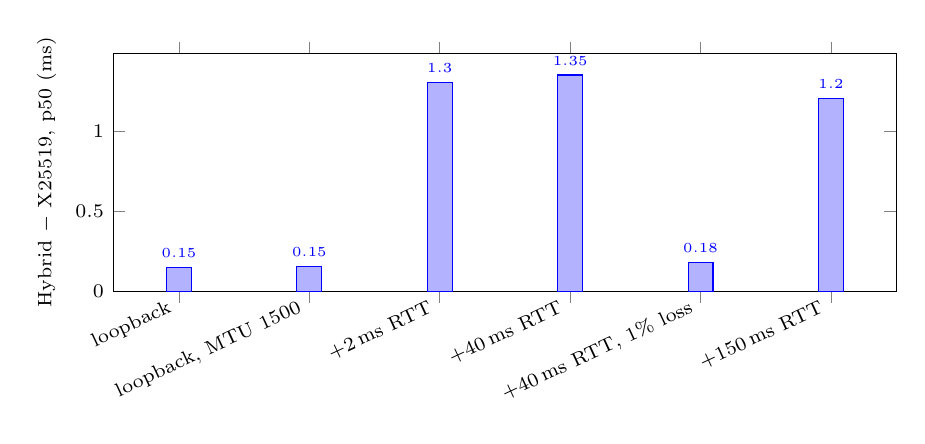
\begin{tikzpicture}
\begin{axis}[
  ybar, ymin=0, width=0.95\linewidth, height=4.6cm, bar width=9pt,
  symbolic x coords={{loopback},{loopback, MTU 1500},{+2\,ms RTT},{+40\,ms RTT},{+40\,ms RTT, 1\% loss},{+150\,ms RTT}}, xtick=data,
  x tick label style={font=\scriptsize, rotate=25, anchor=east},
  y tick label style={font=\scriptsize}, label style={font=\scriptsize},
  ylabel={Hybrid $-$ X25519, p50 (ms)},
  nodes near coords, every node near coord/.append style={font=\tiny, /pgf/number format/.cd, fixed, precision=2},
]
\addplot coordinates {({loopback},0.148) ({loopback, MTU 1500},0.154) ({+2\,ms RTT},1.303) ({+40\,ms RTT},1.349) ({+40\,ms RTT, 1\% loss},0.180) ({+150\,ms RTT},1.204)};
\end{axis}
\end{tikzpicture}

\caption{Extra median handshake time of X25519MLKEM768 over X25519, per
\texttt{netem} profile.}
\label{fig:rq4-extra}
\end{figure}

\paragraph{Latency.} Table~\ref{tab:rq4-tls} and Figure~\ref{fig:rq4-extra}
give the handshake results. On loopback the hybrid handshake's median is
\data{rqfour-loopback-extra} longer than the classical one
(\data{rqfour-loopback-extra-rel}), of the same order as the extra
computation (\data{rqfour-hybrid-kex-extra}). With
added delay the extra median is \data{rqfour-netem-extra-min} to
\data{rqfour-netem-extra-max}, and it does not grow with the round-trip time:
it is \data{rqfour-rtt150ms-extra} at \data{rqfour-rtt150ms-rtt}\,ms, or
\data{rqfour-rtt150ms-extra-rel} of the handshake. We have not isolated why
the extra time is larger with emulated delay than on plain loopback. Under
packet loss the tail is dominated by retransmissions for both clients.
None of the \data{rqfour-docker-handshakes} handshakes in the container
failed, and none of the host's.

\paragraph{Does cost explain non-adoption?} Our measurements suggest not.
At wide-area round-trip times the hybrid key exchange adds at most
\data{rqfour-netem-extra-max} at the median and
\data{rqfour-handshake-bytes-extra} bytes, and the hybrid ClientHello still
fits in a single segment. Go's default client already sends it, and RQ2 shows that
whether a federal endpoint negotiates it depends mostly on who hosts it.
Cost would matter more for post-quantum certificates: an ML-DSA-65 signature
is \data{rqfour-mldsa65-sig-vs-rsa2048} the size of an RSA-2048 one, and no
federal endpoint we measured uses one.
These results describe one machine and emulated links; middleboxes that
mishandle large ClientHellos are not represented.
